%%%%%%%%%%%%%%%%%%%%%%%%%%%%%%%%%%%%%%%%%%%%%%%%%%%%%%%%%%%%%%%%%%%%%%%%%%
%
% Plantilla para libro de texto de matemáticas.
%
% Esta plantilla ha sido desarrollada desde cero, pero utiliza algunas partes
% del código de la plantilla original utilizada en apuntesDGIIM
% (https://github.com/libreim/apuntesDGIIM), basada a su vez en las plantillas
% 'Short Sectioned Assignment' de Frits Wenneker (http://www.howtotex.com),
% 'Plantilla de Trabajo' de Mario Román y 'Plantilla básica de Latex en Español'
% de Andrés Herrera Poyatos (https://github.com/andreshp). También recoge
% ideas de la plantilla 'Multi-Purpose Large Font Title Page' de
% Frits Wenneker y Vel (vel@latextemplates.com).
%
% Licencia:	
% CC BY-NC-SA 4.0 (https://creativecommons.org/licenses/by-nc-sa/4.0/)
%
%%%%%%%%%%%%%%%%%%%%%%%%%%%%%%%%%%%%%%%%%%%%%%%%%%%%%%%%%%%%%%%%%%%%%%%%%

% ---------------------------------------------------------------------------
% CONFIGURACIÓN BÁSICA DEL DOCUMENTO
% ---------------------------------------------------------------------------

%\documentclass[11pt, a4paper, twoside]{article} % Usar para imprimir
\documentclass[10pt, a4paper]{article}

\linespread{1.3}            % Espaciado entre líneas.
\setlength\parindent{0pt}   % No indentar el texto por defecto.
\setlength\parskip{7pt}

% ---------------------------------------------------------------------------
% PAQUETES BÁSICOS
% ---------------------------------------------------------------------------

% IDIOMA
\usepackage[utf8]{inputenc}
\usepackage[spanish, es-tabla, es-lcroman, es-noquoting]{babel}
\usepackage[table,xcdraw]{xcolor}
\usepackage{longtable}
\usepackage{subfigure}

% MATEMÁTICAS
\usepackage{amsmath}    % Paquete básico de matemáticas
\usepackage{amsthm}     % Teoremas
\usepackage{mathrsfs}   % Fuente para ciertas letras utilizadas en matemáticas

% FUENTES
\usepackage{newpxtext, newpxmath}   % Fuente similar a Palatino
\usepackage{FiraSans}                 % Fuente sans serif
\usepackage[T1]{fontenc}
\usepackage[italic]{mathastext}     % Utiliza la fuente del documento
                                    % en los entornos matemáticos

% MÁRGENES
\usepackage[margin=2.5cm, top=3cm]{geometry}

% LISTAS
\usepackage{enumitem}       % Mejores listas
\setlist{leftmargin=.5in}   % Especifica la indentación para las listas.

% Listas ordenadas con números romanos (i), (ii), etc.
\newenvironment{nlist}
{\begin{enumerate}
    \renewcommand\labelenumi{(\emph{\roman{enumi})}}}
  {\end{enumerate}}

%  OTROS
\usepackage[hidelinks]{hyperref}   % Enlaces
\usepackage{graphicx}   % Permite incluir gráficos en el documento
\usepackage{relsize}

% LISTINGS
\usepackage{listings}
\usepackage{xcolor}     % Permite definir y utilizar colores
\usepackage{lipsum}
\usepackage{courier}

% Fijar tabla a posición
\usepackage{array}
\newcolumntype{L}[1]{>{\raggedright\let\newline\\\arraybackslash\hspace{0pt}}m{#1}}
\newcolumntype{C}[1]{>{\centering\let\newline\\\arraybackslash\hspace{0pt}}m{#1}}
\newcolumntype{R}[1]{>{\raggedleft\let\newline\\\arraybackslash\hspace{0pt}}m{#1}}

\setcounter{MaxMatrixCols}{20}

% Colores para los bloques de código
\definecolor{codegreen}{rgb}{0,0.6,0}
\definecolor{codegray}{rgb}{0.5,0.5,0.5}
\definecolor{codepurple}{rgb}{0.58,0,0.82}
\definecolor{backcolour}{rgb}{0.95,0.95,0.92}
\lstdefinestyle{mystyle}{
	backgroundcolor=\color{backcolour!70!white},   
	commentstyle=\color{codegreen},
	keywordstyle=\color{blue},
	numberstyle=\tiny\color{codegray},
	stringstyle=\color{codepurple},
	basicstyle=\footnotesize\ttfamily,
	breakatwhitespace=false,         
	breaklines=true,                 
	captionpos=b,                    
	keepspaces=true,                 
	numbers=left,                    
	numbersep=5pt,                  
	showspaces=false,                
	showstringspaces=false,
	showtabs=false,                  
	tabsize=4
}
\lstset{style=mystyle}

\usepackage{amsmath}
\usepackage{algorithm}


\usepackage[noend]{algpseudocode}

\makeatletter
\def\BState{\State\hskip-\ALG@thistlm}
\makeatother

%\lstset{basicstyle=\footnotesize\ttfamily,breaklines=true}
%\lstset{framextopmargin=50pt,frame=bottomline}
 
% ---------------------------------------------------------------------------
% COMANDOS PERSONALIZADOS
% ---------------------------------------------------------------------------

% \equalto
\newcommand{\verteq}{\rotatebox{90}{$\,=$}}
\newcommand{\equalto}[2]{\underset{\scriptstyle\overset{\mkern4mu\verteq}{#2}}{#1}}


% ---------------------------------------------------------------------------
% COLORES
% ---------------------------------------------------------------------------

\definecolor{50}{HTML}{E0F2F1}
\definecolor{100}{HTML}{B2DFDB}
\definecolor{200}{HTML}{80CBC4}
\definecolor{300}{HTML}{4DB6AC}
\definecolor{400}{HTML}{26A69A}
\definecolor{500}{HTML}{009688}
\definecolor{600}{HTML}{00897B}
\definecolor{700}{HTML}{00796B}
\definecolor{800}{HTML}{00695C}
\definecolor{900}{HTML}{004D40}
\definecolor{ugrColor}{HTML}{c6474b}  % Usado en el título.
\definecolor{ugrColor2}{HTML}{c6474b} % Usado en las secciones.

% ---------------------------------------------------------------------------
% DISEÑO DE PÁGINA
% ---------------------------------------------------------------------------

\usepackage{pagecolor}
\usepackage{afterpage}

% ---------------------------------------------------------------------------
% CABECERA Y PIE DE PÁGINA
% ---------------------------------------------------------------------------

\usepackage{fancyhdr}   % Paquete para cabeceras y pies de página

% Indica que las páginas usarán la configuración de fancyhdr
\pagestyle{fancy}
\fancyhf{}

% Representa la sección de la cabecera
\renewcommand{\sectionmark}[1]{%
\markboth{#1}{}}

% Representa la subsección de la cabecera
\renewcommand{\subsectionmark}[1]{%
\markright{#1}{}}

% Parte derecha de la cabecera
\fancyhead[LE,RO]{\sffamily\textsl{\rightmark} \hspace{1em}  \textcolor{ugrColor2}{\rule[-0.4ex]{0.2ex}{1.2em}} \hspace{1em} \thepage}

% Parte izquierda de la cabecera
\fancyhead[RE,LO]{\sffamily{\leftmark}}

% Elimina la línea de la cabecera
\renewcommand{\headrulewidth}{0pt}

% Controla la altura de la cabecera para que no haya errores
\setlength{\headheight}{14pt}

% ---------------------------------------------------------------------------
% TÍTULOS DE PARTES Y SECCIONES
% ---------------------------------------------------------------------------

\usepackage{titlesec}

% Estilo de los títulos de las partes
\titleformat{\part}[hang]{\Huge\bfseries\sffamily}{\thepart\hspace{20pt}\textcolor{ugrColor}{|}\hspace{20pt}}{0pt}{\Huge\bfseries}
\titlespacing*{\part}{0cm}{-2em}{2em}[0pt]

% Reiniciamos el contador de secciones entre partes (opcional)
\makeatletter
\@addtoreset{section}{part}
\makeatother

% Estilo de los títulos de las secciones, subsecciones y subsubsecciones
\titleformat{\section}
  {\Large\bfseries\sffamily}{\thesection}{1em}{}

\titleformat{\subsection}
  {\Large\sffamily}{\thesubsection}{1em}{}[\vspace{.5em}]

\titleformat{\subsubsection}
  {\sffamily}{\thesubsubsection}{1em}{}

% ---------------------------------------------------------------------------
% ENTORNOS PERSONALIZADOS
% ---------------------------------------------------------------------------

\usepackage{mdframed}

%% DEFINICIONES DE LOS ESTILOS

% Nuevo estilo para definiciones
\newtheoremstyle{definition-style}  % Nombre del estilo
{}                                  % Espacio por encima
{}                                  % Espacio por debajo
{}                                  % Fuente del cuerpo
{}                                  % Identación
{\bf\sffamily}                      % Fuente para la cabecera
{.}                                 % Puntuación tras la cabecera
{.5em}                              % Espacio tras la cabecera
{\thmname{#1}\thmnumber{ #2}\thmnote{ (#3)}}  % Especificación de la cabecera

% Nuevo estilo para notas
\newtheoremstyle{remark-style}
{10pt}
{10pt}
{}
{}
{\itshape \sffamily}
{.}
{.5em}
{}

% Nuevo estilo para teoremas y proposiciones
\newtheoremstyle{theorem-style}
{}
{}
{}
{}
{\bfseries \sffamily}
{.}
{.5em}
{\thmname{#1}\thmnumber{ #2}\thmnote{ (#3)}}

% Nuevo estilo para teoremas y proposiciones
\newtheoremstyle{theorem2-style}
{}
{}
{}
{}
{\bfseries \sffamily}
{.}
{.5em}
{\thmname{#1}\thmnote{ (#3)}}

% Nuevo estilo para ejemplos
\newtheoremstyle{example-style}
{10pt}
{10pt}
{}
{}
{\bf \sffamily}
{}
{.5em}
{\thmname{#1}\thmnumber{ #2.}\thmnote{ #3.}}

% Nuevo estilo para la demostración

\makeatletter
\renewenvironment{proof}[1][\proofname] {\par\pushQED{\qed}\normalfont\topsep6\p@\@plus6\p@\relax\trivlist\item[\hskip\labelsep\itshape\sffamily#1\@addpunct{.}]\ignorespaces}{\popQED\endtrivlist\@endpefalse}
\makeatother

%% ASIGNACIÓN DE LOS ESTILOS

% Teoremas, proposiciones y corolarios
\newtheoremstyle{theorem-style}{}{}{}{}{}{}{ }{}
\theoremstyle{theorem-style}
\newtheorem*{datos}{}
\theoremstyle{theorem-style}
\newtheorem{nth}{Teorema}[section]
\newtheorem{nprop}{Proposición}[section]
\newtheorem{ncor}{Corolario}[section]
\newtheorem{lema}{Lema}[section]
\theoremstyle{theorem2-style}
\newtheorem{demostracion}{\textbf{\emph{Demostración}}}

% Definiciones
\theoremstyle{definition-style}
\newtheorem{ndef}{Definición}[section]

% Notas
\theoremstyle{remark-style}
\newtheorem*{nota}{Nota}

% Ejemplos
\theoremstyle{example-style}
\newtheorem{ejemplo}{Ejemplo}[section]

% Ejercicios y solución
\theoremstyle{definition-style}
\newtheorem{ejer}{Ejercicio}[section]

\theoremstyle{remark-style}
\newtheorem*{sol}{Solución}

\theoremstyle{remark-style}
\newtheorem*{dem}{Demostración}

%% MARCOS DE LOS ESTILOS

% Configuración general de mdframe, los estilos de los teoremas, etc
\mdfsetup{
  skipabove=1em,
  skipbelow=1em,
  innertopmargin=1em,
  innerbottommargin=1em,
  splittopskip=2\topsep,
}

% Definimos los marcos de los estilos


\mdfdefinestyle{datos-frame}{
	linewidth=2pt, %
	linecolor= ugrColor, %
	topline=false, %
	bottomline=false, %
	rightline=false,%
	leftmargin=0em, %
	innerleftmargin=1em, %
	innerrightmargin=1em,
	rightmargin=0em, %
}%
\mdfdefinestyle{nth-frame}{
	linewidth=2pt, %
	linecolor= 500, %
	topline=false, %
	bottomline=false, %
	rightline=false,%
	leftmargin=0em, %
	innerleftmargin=1em, %
  innerrightmargin=1em,
	rightmargin=0em, %
}%

\mdfdefinestyle{nprop-frame}{
	linewidth=2pt, %
	linecolor= 300, %
	topline=false, %
	bottomline=false, %
	rightline=false,%
	leftmargin=0pt, %
	innerleftmargin=1em, %
	innerrightmargin=1em,
	rightmargin=0pt, %
}%

\mdfdefinestyle{dem_mia-frame}{
	linewidth=2pt, %
	linecolor= ugrColor, %
	topline=false, %
	bottomline=false, %
	rightline=false,%
	leftmargin=0pt, %
	innerleftmargin=1em, %
	innerrightmargin=1em,
	rightmargin=0pt, %
}%

\mdfdefinestyle{ndef-frame}{
	linewidth=2pt, %
	linecolor= 500, %
	backgroundcolor= 50,
	topline=false, %
	bottomline=false, %
	rightline=false,%
	leftmargin=0pt, %
	innerleftmargin=1em, %
	innerrightmargin=1em,
	rightmargin=0pt, %
}%

\mdfdefinestyle{ejer-frame}{
	linewidth=2pt, %
	linecolor= ugrColor, %
	backgroundcolor= 50,
	topline=false, %
	bottomline=false, %
	rightline=false,%
	leftmargin=0pt, %
	innerleftmargin=1em, %
	innerrightmargin=1em,
	rightmargin=0pt, %
}%

\mdfdefinestyle{ejemplo-frame}{
	linewidth=0pt, %
	linecolor= 300, %
	leftline=false, %
	rightline=false, %
	leftmargin=0pt, %
	innerleftmargin=1.3em, %
	innerrightmargin=1em,
	rightmargin=0pt, %
	innertopmargin=0em,%
	innerbottommargin=0em, %
	splittopskip=\topskip, %
}%

% Asignamos los marcos a los estilos
\surroundwithmdframed[style=nth-frame]{nth}
\surroundwithmdframed[style=datos-frame]{datos}
\surroundwithmdframed[style=nprop-frame]{nprop}
\surroundwithmdframed[style=nprop-frame]{ncor}
\surroundwithmdframed[style=ndef-frame]{ndef}
\surroundwithmdframed[style=ejer-frame]{ejer}
\surroundwithmdframed[style=ejemplo-frame]{ejemplo}
\surroundwithmdframed[style=ejemplo-frame]{sol}
\surroundwithmdframed[style=dem_mia-frame]{demostracion}

% ---------------------------------------------------------------------------
% CONFIGURACIÓN DE LA PORTADA
% ---------------------------------------------------------------------------

\newcommand{\asignatura}{Metaheurísticas}
\newcommand{\universidad}{Universidad de Granada}

% ---------------------------------------------------------------------------
% FOTO DE LA PORTADA
% ---------------------------------------------------------------------------




\title{\vspace{3cm}\textcolor{ugrColor}{\textbf{{{{\Huge Aprendizaje de Pesos en Características}}}}}}

\usepackage{tcolorbox}
\newtcolorbox{example}[2][]
{colback=ugrColor!25!white,colframe=ugrColor!90!white,
fonttitle=\bfseries, title=Enunciado~\thetcbcounter: #2,#1}

\usepackage{titling}
\include{titlepage}
\usepackage{wallpaper}
\date{12 de mayo 2022}

\usepackage{graphicx}
\begin{document}
\ThisULCornerWallPaper{1}{ugrA4.pdf}
\maketitle

\begin{center}
\large
\vspace{2cm}
\textbf{\emph{\Large Metaheurísticas}}\\
\emph{\large Gallego Menor, Francisco Javier}\\
\emph{\large javigallego@correo.ugr.es}\\
\emph{\large 74745747W}\\

\end{center}
              
\newpage


\tableofcontents
\newpage

\section{Introducción}
El problema de clasificación consiste en, dado un conjunto $A=\{(a,b) \ : a \in R^n, b \ es \ una \ clase\}$ de datos ya clasificados, obtener un sistema que permita clasificar un objeto nuevo de forma automática.\\

 Un ejemplo de clasificador, y el que utilizaremos en esta práctica,es el $k-NN$ , $k$ vecinos más cercanos. Este toma la clase que más se repita entre los $u_i\in A$ tales que su distancia al nuevo elemento $u$ sea mínima. En nuestro caso, en una versión sencilla del problema, consideraremos el clasificador $1-NN$. \\

Consideraremos como distancias la distancia trivial si las características son discretas (esto es, la distancia será 1 si las características son diferentes, y 0 si son iguales. La denotamos como $d_n$), y la distancia euclídea para características que sean continuas. Además, cada característica tendrá un peso asociado, por lo que dado un vector de pesos $w$, la distancia entre dos vectores $u$ y $v$ será de la forma:
\[
d(u,v) = \sqrt {\sum_i w_i(u_i- v_i)^2 + \sum_j w_j d_n(u_j,v_j)}
\]

 El aprendizaje de pesos en características consiste  en hallar un vector de pesos que maximice la siguiente función:
\[
F(w) = \alpha T_{clas}(w) + (1-\alpha)T_{red}(w)
\]
Donde
\begin{itemize}
\item $T_{clas}$ es la función que indica cómo de bueno es nuestro clasificador, es decir, cuántos casos ha clasificado correctamente si entrenamos el clasificador usando el resto de datos ,la técnica \emph{k-fold cross validation}, y dejando un elemento fuera (leave one out).
	\item $T_{red}$ que es la función que nos indica cuántas características de un dato tienen un peso menor que un valor establecido, en nuestro caso $0.2$.
\end{itemize}


\section{Descripción de la aplicación de los algoritmos}

\subsection{Esquemas de representación}
\textcolor{ugrColor}{Antes de comenzar, comentar brevemente que aquellas secciones que no añaden nada nuevo (aquellas cogidas de la P1) las marco en rojo}. En nuestro problema, los datos de entrada poseen los elementos que siguen: 
\begin{itemize}	
	\item \textbf{Clase del elemento (target)}: que es la categoría a la que corresponde el mismo, dependiendo de cada dataset
	\item \textbf{Ejemplo}: que es un par que tiene un vector de features y una clase (target).
	\item \textbf{Dataset}: que contendrá una lista de ejemplos
	\item \textbf{Vector de características}: vector de valores reales que trataremos de normalizar al intervalo $[0,1]$ para trabajar con ellos.	

\end{itemize}
A partir de los elementos previamente descritos, vamos a obtener nuestra solución al problema. Esta consistirá en un vector de pesos, cuyos valores reales se encontrarán también en el intervalo $[0,1]$.

\subsection{Operadores comunes}
En esta sección, procederemos a describir aquellas funcionalidades que sean comunes para todos los algoritmos. En nuestro caso, solo es la que sigue: 

\subsubsection{Generación Soluciones Aleatorias}

Para la generación de las soluciones aleatorias usamos \textbf{np.random.uniform}, el cual implica que cualquier valor dentro del intervalo dado tiene la misma probabilidad de ser extraído por uniforme. En nuestro caso el [0,1). El pseudocódigo es el siguiente: \\

\begin{algorithmic}[1]
\Procedure{Crear Solución Aleatoria}{}:
\State vector de pesos $\gets$ np.random.uniform(extremo inferior intervalo, extremo superior, longitud del vector)
\EndProcedure
\end{algorithmic}

VERIFICAR ESTO. NO ES COMUN A TODOS PORQUE HAY ALGUNOS QUE NO LOS USAN .

\subsubsection{\textcolor{ugrColor}{Mutación}}
Este operador es común para todos los algoritmos de la práctica. Al mutar, sumaremos a la componente $j-esima$ un valor aleatorio y truncaremos al intervalo $[0,1]$ si el nuevo valor se nos escapara del intervalo:\\
\begin{algorithmic}[1]
\Procedure{mute}{w,sigma,j}
\State $w(j) \gets w(j) + random(0,1, scale = sigma)$
\State $w(j) \gets Normalize(w(j))$
\State \textbf{return} w
\EndProcedure
\end{algorithmic}

\subsection{Función objetivo}
En nuestro caso, se nos indica que tomemos como $alpha$ el valor $0.5$, así que en realidad lo que estamos haciendo es:
\[
F = 0.5(T_{clas} + T_{red})
\]
Hemos modificado la forma de calcular  $T_{class}$ con respecto a su versión de la P1, pues era el cuello de botella en la ejecución. La calcularemos de la siguiente manera ahora:\\

\begin{algorithmic}[1]
\Procedure{T-class}{w, features, targets}
\State dataw $\gets$ features * w
\State classifier $\gets$ clasificador 1-NN de Sklearn
\State Entrenamos el modelo
\State ind\_near $\gets$ indice vecino mas cercano
\State tasa\_class $\gets$ media (targets[ind\_near] == targets)
\State \textbf{return} tasa\_class / 100

\EndProcedure
\end{algorithmic}

Y calcularemos $T_{red}$ así:\\
\begin{algorithmic}[1]
\Procedure{T-red}{weight}
\State \textbf{return} (Nº Pesos < 0.2) / Nº Pesos Totales
\EndProcedure
\end{algorithmic}

\section{Descripción de los algoritmos considerados}

\subsection{\textcolor{ugrColor}{Algoritmo Greedy Relief}}
El algoritmo de Greedy Relief se encarga de recorrer todo el conjunto de datos, muestra por muestra. En cada uno de ellos, dependiendo del amigo y enemigo más cercanos, hace una modificación del vector de pesos. Entonces, lo que haremos será: por cada una de las muestras, obtener un conjunto de datos amigos (que pertenecen a su misma clase) y uno de enemigos (no pertenecen a su misma clase). Posteriormente, obtendremos el vecino más cercano de cada uno de ellos. \\

\begin{algorithm}
\caption{Greedy Relief}\label{euclid}
\begin{algorithmic}[1]
\Procedure{greedyRelief}{features, targets}
\State $w \gets [0, ...., 0]$
\State distances $\gets$ matriz cuadrada de distancias (euclídeas)
\BState \textbf{\emph{loop}:} para cada muestra del conjunto de entrenamiento

\State en\_indices $\gets$ índices de ejemplos con distinto target a la muestra

\State fr\_indices $\gets$ índices de ejemplos con igual target a la muestra

\State friends $\gets$ features[fr\_indices]
\State enemies $\gets$ features[en\_indices]
\State
\State closestFriend $\gets$ Amigo mas cercano
\State closestEnemy $\gets$ Enemigo mas cercano
\State
\State w $\gets$ w + |features(i) - closestEnemy| - |features(i)-closestFriend|
\BState \textbf{\emph{endloop}}
\State w $\gets$ Truncamos valores negativos a 0
\State w $\gets$ Normalizamos w
\State \textbf{return} w
\EndProcedure
\end{algorithmic}
\end{algorithm}

\subsection{\textcolor{ugrColor}{Búsqueda local}}
Para este algoritmo, debemos definir el algoritmo que hemos usado para obtener una mutación de un ejemplo. Al mutar, sumaremos a la componente $j-esima$ un valor aleatorio y truncaremos al intervalo $[0,1]$ si el nuevo valor se nos escapara del intervalo:
\begin{algorithmic}[1]
\Procedure{mute}{w,sigma,j}
\State $w(j) \gets w(j) + random(0,1)$
\State $w(j) \gets Normalize(w(j))$
\State \textbf{return} w
\EndProcedure
\end{algorithmic}
En el procedimiento de cálculo de pesos mediante la búsqueda local intervendrá la función de evaluación, que será notada por $f(w)$.

Así, el procedimiento general para la generación de pesos para la búsqueda local sería:


\begin{algorithm}
\caption{Local Search}\label{euclid}
\begin{algorithmic}[1]
\Procedure{localSearch}{initialWeight,features,targets}
\State weight $\gets$ valor inicial para los pesos
\State bestF $\gets$ valor inicial para la función objetivo
\State index $\gets$ Ordenación de forma aleatoria de los índices
\State improve $\gets$ False
\BState \textbf{\emph{while}}  (menos evaluaciones que 15000) and (Haya mejora antes de generar 20*n vecinos) 

\State w $\gets$ vector de pesos mutando componente j-esima

\State newF $\gets$ Valor funcion objetivo para w
\If {newF $>$ bestF}

bestF $\gets$ newF

weight $\gets$ w

notMuted $\gets$ 0

improve $\gets$ True

\Else

notMuted $\gets$ notMuted + 1

\EndIf

\State evaluaciones $\gets$ evaluaciones +1

\If {(Hay mejora) or (Todos los componentes han sido ya mutados)}

improve $\gets$ False

index $\gets$ Ordenación de forma aleatoria de los índices

\EndIf

\BState \emph{endloop}
\State \textbf{return} weight
\EndProcedure
\end{algorithmic}
\end{algorithm}

\pagebreak
\subsection{Búsqueda Multiarranque Básica (BMB)}

Es el algoritmo multiarranque más básico que podemos considerar. En él,  las soluciones iniciales se generan al azar, y la etapa de búsqueda se realiza
mediante el algoritmo de Búsqueda Local. Siguiendo el pseudocódigo de los seminarios y teoría, se ha implementado una versión concisa aprovechando la búsqueda local implementada en las sesiones anteriores.
\vspace{0.2cm}

\begin{algorithm}
\caption{BMB}\label{euclid}
\begin{algorithmic}[1]
\Procedure{BMB}{data,classes, trainIndex, testIndex}
\State ini\_weights $\gets$ generamos la solución inicial
\State bestF $\gets$ f(ini\_weights)
\State
\BState \textbf{\emph{for i in}}
(range(15)):
\State w $\gets$ localSearch(ini\_weights, data, classes) \hspace{3cm}(15000 / 15 evaluaciones)

\State currentF $\gets$ f(w)
\State
\If {currentF > bestF}
\State weights $\gets$ np.copy(w)
\State bestF $\gets$ currentF
\EndIf
\State
\State ini\_weights $\gets$ generamos nueva solución aleatoria inicial

\BState \emph{endloop}
\State Entrenamos el modelo, predecimos y calculamos las tasas
\State \textbf{return} tasa clasificación, tasa reducción
\EndProcedure
\end{algorithmic}
\end{algorithm}

\subsection{Enfriamiento Simulado}

Este algoritmo es bastante más complejo que el anterior. Empezamos comentando algunas particularidades. Para el cálculo de la temperatura inicial se sigue el siguiente esquema: $T_0 = 0.3 * f(inicial) / -ln(0.3)$. Donde $f(x)$ es nuestra función fitness. La temperatura inicial se calcula como el mínimo entre $10^{-3}$ y $T_0$, para que nunca sea la temperatura final mayor que la inicial.

Por otro lado, existen varios criterios de parada. Para el bucle externo el criterio de parada es el número de evaluaciones de la función fitness y la temperatura actual. Mientras que en el bucle interno es el número de vecinos generados y el número de soluciones aceptadas (entre cada enfriamiento).

Finalmente el criterio de enfriamiento es Cauchy modificado donde tenemos que $T_{i+1} = T_i / (1 + \beta * T_i)$, para $\beta = (T_0 - T_f) / (M * T_0 * T_f)$. M es el número de enfriamientos a realizar, es decir el número máximo de evaluaciones a la función fitness, entre el número de vecinos que se genera en cada bucle interno. 

\begin{algorithm}
\caption{ES}\label{euclid}
\begin{algorithmic}[1]
\Procedure{ES}{data,classes, trainIndex, testIndex}
\State weights $\gets$ generamos la solución inicial
\State bestF, currentF $\gets$ f(weights)
\State best\_weights $\gets$ weights.copy()
\State

\State max\_neighbours $\gets$ 10 * nº features
\State max\_successes $\gets$ 0.1 * max\_neighbours
\State M $\gets$ nº de enfriamientos a realizar
\State
\State $T_0 \gets$ $\frac{0.3\hspace{0.1cm}*\hspace{0.1cm}currentF}{- \log(0.3)}$
\State $T_F \gets$ $10^{-3}$
\State $\beta \gets \frac{T_0 - T_F}{M * T_0 * T_F}$ 
\State $T_current \gets T_0$
\State
\BState \textbf{\emph{while}}
max\_successes > 0 and $T_{current} > T_F$ and coolings < M
\State neighbours, num\_successes $\gets$ 0

\State \textbf{\emph{while}} num\_successes < max\_successes and negihbours < max\_neighbours

\State \hspace{0.75cm}w $\gets$ weights.copy()
\State \hspace{0.75cm}index $\gets$ componente aleatoria
\State \hspace{0.75cm}w $\gets$ mute(w, index)
\State \hspace{0.75cm}newF $\gets$ f(w)

\State \hspace{0.75cm}$\Delta f$ $\gets$ newF - currentF

\State
\State \hspace{0.75cm}\textbf{if} diff > 0 or U(0,1) $\leq e^{\frac{\Delta f}{T_{current}}}$  \textbf{then}

\State \hspace{1.25cm}currentF $\gets$ newF
\State \hspace{1.25cm}num\_successes $\gets$ +1
\State \hspace{1.25cm}weights $\gets$ w.copy()
\State \hspace{1.25cm}\textbf{if} currentF > bestF \textbf{then} 

\State \hspace{1.75cm}best\_weights $\gets$ weights
\State \hspace{1.75cm}bestF $\gets$ currentF

\State \hspace{1.25cm}neighbours $\gets$ +1

\State \textbf{\emph{endloop}}

\State $T_{current} = \frac{T_{current}}{1+\beta * T_{current}}$
\State coolings $\gets$ +1

\BState \emph{endloop}
\State Entrenamos el modelo, predecimos y calculamos las tasas
\State \textbf{return} tasa clasificación, tasa reducción
\EndProcedure
\end{algorithmic}
\end{algorithm}

\subsection{Búsqueda Local Iterativa}

La ILS está basada en la aplicación repetida de la Búsqueda Local a una solución inicial que se obtiene por mutación de un óptimo local previamente encontrado. Siguiendo el pseudocódigo de los seminarios y teoría, se ha implementado una versión concisa aprovechando la búsqueda local implementada en las sesiones anteriores.
\vspace{0.2cm}

\begin{algorithm}
\caption{ILS}\label{euclid}
\begin{algorithmic}[1]
\Procedure{ILS}{data,classes, trainIndex, testIndex}
\State weights $\gets$ generamos la solución inicial
\State bestF, currentF $\gets$ f(weights)
\State best\_weigths $\gets$ weights.copy()
\State mutations $\gets$ range(0.1 * nº features)
\State
\BState \textbf{\emph{for i in}}
(range(15)):
\State \hspace{0.5cm}\emph{for} i in mutations

\State \hspace{1cm}index $\gets$ índice característica aleatoria

\State \hspace{1cm}weigths $\gets$ mute(weights, index, 0.4)
\State \hspace{0.5cm}\emph{endloop}
\State \hspace{0.5cm}weights $\gets$ aplicamos búsqueda local para 15000 / 15 evaluaciones máximas
\State \hspace{0.5cm}currentF $\gets$ f(weights)

\State \hspace{0.5cm}\textbf{if} currentF > bestF  \textbf{then}
\State \hspace{1cm}bestF $\gets$ currentF
\State \hspace{1cm}best\_weights $\gets$ weights
\State
\State \hspace{0.5cm}weights $\gets$ best\_weights.copy()
\BState \emph{endloop}
\State Entrenamos el modelo, predecimos y calculamos las tasas
\State \textbf{return} tasa clasificación, tasa reducción
\EndProcedure
\end{algorithmic}
\end{algorithm}

\pagebreak
\subsection{Híbrido ILS - ES}

Basicamente se repite el mismo pseudocodigo pero cambiando la localSearch por el enfriamiento simulado. 

\begin{algorithm}
\caption{ILS}\label{euclid}
\begin{algorithmic}[1]
\Procedure{ILS}{data,classes, trainIndex, testIndex}
\State weights $\gets$ generamos la solución inicial
\State bestF, currentF $\gets$ f(weights)
\State best\_weigths $\gets$ weights.copy()
\State mutations $\gets$ range(0.1 * nº features)
\State
\BState \textbf{\emph{for i in}}
(range(15)):
\State \hspace{0.5cm}\emph{for} i in mutations

\State \hspace{1cm}index $\gets$ índice característica aleatoria

\State \hspace{1cm}weigths $\gets$ mute(weights, index, 0.4)
\State \hspace{0.5cm}\emph{endloop}
\State \hspace{0.5cm}weights $\gets$ aplicamos el enfriamiento simulado para 15000 / 15 evaluaciones máximas
\State \hspace{0.5cm}currentF $\gets$ f(weights)

\State \hspace{0.5cm}\textbf{if} currentF > bestF  \textbf{then}
\State \hspace{1cm}bestF $\gets$ currentF
\State \hspace{1cm}best\_weights $\gets$ weights
\State
\State \hspace{0.5cm}weights $\gets$ best\_weights.copy()
\BState \emph{endloop}
\State Entrenamos el modelo, predecimos y calculamos las tasas
\State \textbf{return} tasa clasificación, tasa reducción
\EndProcedure
\end{algorithmic}
\end{algorithm}

\newpage
\section{Procedimiento considerado para desarrollar la práctica}
Para desarrollar la práctica, he usado \textbf{Python} como lenguaje de programación, sin usar ningún framework de metaheurísticas.

Para poder ejecutar el código , hace falta tener instalado \emph{Numpy, Scipy} y \emph{Sklearn}. Este último es muy útil para la realización de prácticas de este estilo pues trae implementaciones de muchas funcionalidades básicas para \emph{Machine learning}.

El fichero que hay que ejecutar dentro de la carpeta es el fichero \emph{\textbf{main.py}}. Para ello, basta con escribir en la terminal:
\[
\textit{python main.py}
\]
Tras la ejecución, comenzará a ejecutar los algoritmos sobre los 3 ficheros de datos que tenemos, que se explicarán más adelante.

La lista de archivos que contiene la práctica son los siguientes:
\begin{itemize}
	\item \textbf{main.py}: fichero principal a ejecutar para la ejecución de nuestro programa.	
	\item \textbf{algorithms.py}: fichero en el que se encuentran los algoritmos de la P1, y algunas funciones auxiliares programadas para la práctica.
\item \textbf{P3\_algorithms.py}: fichero con los algoritmos implementados en esta práctica. 
	\item \textbf{graficas.ipynb}: notebook mediante el cual he generado las gráficas.  
	\item \textbf{Datasets}: carpeta en la que se encuentran los datasets almacenados.
	\item \textbf{Archivos\_CSV}: carpeta con los archivos CSV necesarios para agilizar el proceso de creación de las gráficas.
	
\end{itemize}
\newpage
\section{Experimentos y análisis de resultados}

\subsection{Resultados de cada algoritmo}

\textbf{Algoritmo 1-NN}

\begin{table}[ht!]
\begin{tabular}{ccccc|cccc|cccc}
\centering
 & \multicolumn{4}{c}{\textit{Ionosphere}} & \multicolumn{4}{c}{\textit{Parkinson}} & \multicolumn{4}{c}{\textit{Spectf-Heart}} \\ \hline
\textbf{Nº} & \textbf{Clas} & \textbf{Red} & \textbf{Agr} & \textbf{T} & \textbf{Clas} & \textbf{Red} & \textbf{Agr} & \textbf{T} & \textbf{Clas} & \textbf{Red} & \textbf{Agr} & \textbf{T} \\ \hline
0&	 0.85 & 0.00 & 0.42 & 0.00283 & 	0.72 & 0.00 & 0.36 & 0.00099 & 		0.97 & 0.00 & 0.49 & 0.00309 \\ 
1&	 0.77 & 0.00 & 0.39 & 0.00276 & 	0.82 & 0.00 & 0.41 & 0.00100 & 		0.90 & 0.00 & 0.45 & 0.00323 \\ 
2&	 0.83 & 0.00 & 0.41 & 0.00279 & 	0.95 & 0.00 & 0.47 & 0.00100 & 		0.71 & 0.00 & 0.36 & 0.00312 \\ 
3&	 0.91 & 0.00 & 0.46 & 0.00278 & 	0.74 & 0.00 & 0.37 & 0.00100 & 		0.77 & 0.00 & 0.39 & 0.00317 \\ 
4&	 0.86 & 0.00 & 0.43 & 0.00285 & 	0.67 & 0.00 & 0.33 & 0.00101 & 		0.99 & 0.00 & 0.49 & 0.00307 \\ 
\hline
Media&	 0.84 & 0.00 & 0.42 & 0.00280	& 0.78 & 0.00 & 0.39 & 0.00100	& 0.87 & 0.00 & 0.43 & 0.00314
 \\ Std&	 0.05 & 0.00 & 0.02 & 0.00003	& 0.10 & 0.00 & 0.05 & 0.00001	&	0.11 & 0.00 & 0.05 & 0.00006
 \\ 
\end{tabular}
\end{table}


\textbf{Algoritmo RELIEF}

\begin{table}[ht!]
\begin{tabular}{ccccc|cccc|cccc}
\centering
 & \multicolumn{4}{c}{\textit{Ionosphere}} & \multicolumn{4}{c}{\textit{Parkinson}} & \multicolumn{4}{c}{\textit{Spectf-Heart}} \\ \hline
\textbf{Nº} & \textbf{Clas} & \textbf{Red} & \textbf{Agr} & \textbf{T} & \textbf{Clas} & \textbf{Red} & \textbf{Agr} & \textbf{T} & \textbf{Clas} & \textbf{Red} & \textbf{Agr} & \textbf{T} \\ \hline
0&	 0.86 & 0.03 & 0.44 & 0.01278 & 	0.72 & 0.05 & 0.38 & 0.00627 & 		0.97 & 0.11 & 0.54 & 0.01284 \\ 
1&	 0.79 & 0.03 & 0.41 & 0.01250 & 	0.82 & 0.00 & 0.41 & 0.00475 & 		0.91 & 0.00 & 0.46 & 0.01303 \\ 
2&	 0.80 & 0.09 & 0.44 & 0.01248 & 	0.95 & 0.05 & 0.50 & 0.00474 & 		0.74 & 0.00 & 0.37 & 0.01291 \\ 
3&	 0.91 & 0.03 & 0.47 & 0.01277 & 	0.69 & 0.05 & 0.37 & 0.00474 & 		0.74 & 0.00 & 0.37 & 0.01297 \\ 
4&	 0.86 & 0.03 & 0.44 & 0.01278 & 	0.67 & 0.00 & 0.33 & 0.00476 & 		0.99 & 0.09 & 0.54 & 0.01274 \\ 
\hline
Media&	 0.84 & 0.04 & 0.44 & 0.01266	& 0.77 & 0.03 & 0.40 & 0.00505		&0.87 & 0.04 & 0.46 & 0.01290
 \\ Std&	 0.05 & 0.02 & 0.02 & 0.00014	&0.10 & 0.02 & 0.06 & 0.00061	&	0.11 & 0.05 & 0.08 & 0.00010
 \\

\end{tabular}
\end{table}

\textbf{Algoritmo de búsqueda local}

\begin{table}[ht!]
\begin{tabular}{ccccc|cccc|cccc}
\centering
 & \multicolumn{4}{c}{\textit{Ionosphere}} & \multicolumn{4}{c}{\textit{Parkinson}} & \multicolumn{4}{c}{\textit{Spectf-Heart}} \\ \hline
\textbf{Nº} & \textbf{Clas} & \textbf{Red} & \textbf{Agr} & \textbf{T} & \textbf{Clas} & \textbf{Red} & \textbf{Agr} & \textbf{T} & \textbf{Clas} & \textbf{Red} & \textbf{Agr} & \textbf{T} \\ \hline

0&	 0.89 & 0.79 & 0.84 & 2.47617 & 	0.77 & 0.68 & 0.73 & 0.54792 & 		0.97 & 0.84 & 0.91 & 3.52364 \\ 
1&	 0.87 & 0.85 & 0.86 & 2.03225 & 	0.85 & 1.00 & 0.92 & 1.16207 & 		0.89 & 0.86 & 0.87 & 4.97461 \\ 
2&	 0.86 & 0.76 & 0.81 & 1.77548 & 	0.87 & 0.82 & 0.84 & 0.81054 & 		0.74 & 0.91 & 0.83 & 3.02352 \\ 
3&	 0.97 & 0.97 & 0.97 & 2.93292 & 	0.74 & 1.00 & 0.87 & 1.17324 & 		0.80 & 0.82 & 0.81 & 2.94800 \\ 
4&	 0.86 & 0.88 & 0.87 & 1.89319 & 	0.62 & 0.91 & 0.76 & 0.53875 & 		0.99 & 0.68 & 0.83 & 3.57642 \\
\hline 
Media&	 0.89 & 0.85 & 0.87 & 2.22200	&0.77 & 0.88 & 0.83 & 0.84650	&	0.88 & 0.82 & 0.85 & 3.60924
 \\ Std&	 0.04 & 0.07 & 0.05 & 0.42744	&0.09 & 0.12 & 0.07 & 0.27982	&	0.09 & 0.08 & 0.04 & 0.72841
 \\  

\end{tabular}
\end{table}
\pagebreak
\textbf{BMB}

\begin{table}[ht!]
\begin{tabular}{ccccc|cccc|cccc}
\centering
 & \multicolumn{4}{c}{\textit{Ionosphere}} & \multicolumn{4}{c}{\textit{Parkinson}} & \multicolumn{4}{c}{\textit{Spectf-Heart}} \\ \hline
\textbf{Nº} & \textbf{Clas} & \textbf{Red} & \textbf{Agr} & \textbf{T} & \textbf{Clas} & \textbf{Red} & \textbf{Agr} & \textbf{T} & \textbf{Clas} & \textbf{Red} & \textbf{Agr} & \textbf{T} \\ \hline
0&	 0.86 & 0.91 & 0.89 & 28.95681 & 	0.77 & 1.00 & 0.88 & 10.89507 & 0.94 & 0.86 & 0.90 & 23.11825 \\ 
1&	 0.84 & 0.91 & 0.88 & 23.07019 & 	0.77 & 1.00 & 0.88 & 10.65365 & 0.91 & 0.89 & 0.90 & 19.02795 \\ 
2&	 0.77 & 0.88 & 0.83 & 19.34851 & 	0.95 & 1.00 & 0.97 & 10.32327 & 0.73 & 0.95 & 0.84 & 18.88538 \\ 
3&	 0.91 & 0.97 & 0.94 & 19.68961 & 	0.77 & 1.00 & 0.88 & 11.13045 & 0.80 & 0.86 & 0.83 & 19.26337 \\ 
4&	 0.91 & 0.91 & 0.91 & 17.38932 & 	0.62 & 1.00 & 0.81 & 10.89773 & 0.96 & 0.84 & 0.90 & 19.06175 \\ 
\hline
Media&	 0.86 & 0.92 & 0.89 & 21.69089	& 0.77 & 1.00 & 0.89 & 10.78003	&	0.87 & 0.88 & 0.88 & 19.87134
 \\ Std&	 0.05 & 0.03 & 0.04 & 4.06673&	0.11 & 0.00 & 0.05 & 0.27367	&	0.09 & 0.04 & 0.03 & 1.62794
 \\ 
\end{tabular}
\end{table}

\textbf{ES}

\begin{table}[ht!]
\begin{tabular}{ccccc|cccc|cccc}
\centering
 & \multicolumn{4}{c}{\textit{Ionosphere}} & \multicolumn{4}{c}{\textit{Parkinson}} & \multicolumn{4}{c}{\textit{Spectf-Heart}} \\ \hline
\textbf{Nº} & \textbf{Clas} & \textbf{Red} & \textbf{Agr} & \textbf{T} & \textbf{Clas} & \textbf{Red} & \textbf{Agr} & \textbf{T} & \textbf{Clas} & \textbf{Red} & \textbf{Agr} & \textbf{T} \\ \hline
0&	 0.92 & 0.94 & 0.93 & 5.56628 & 	0.74 & 0.95 & 0.85 & 2.19462 & 0.96 & 0.89 & 0.92 & 3.77431 \\ 
1&	 0.86 & 0.97 & 0.91 & 4.60594 & 	0.82 & 0.95 & 0.89 & 2.13416 & 0.86 & 0.82 & 0.84 & 3.13027 \\ 
2&	 0.81 & 0.94 & 0.88 & 3.79682 & 	0.87 & 0.95 & 0.91 & 2.08432 & 0.79 & 0.91 & 0.85 & 3.02167 \\ 
3&	 0.89 & 0.97 & 0.93 & 3.13974 & 	0.67 & 0.95 & 0.81 & 2.05098 & 0.93 & 0.89 & 0.91 & 2.96716 \\ 
4&	 0.91 & 0.97 & 0.94 & 3.11074 & 	0.67 & 0.95 & 0.81 & 1.87637 & 0.97 & 0.80 & 0.88 & 3.05440 \\
\hline 
Media&	 0.88 & 0.96 & 0.92 & 4.04391	& 0.75 & 0.95 & 0.85 & 2.06809	&	0.90 & 0.86 & 0.88 & 3.18956
 \\ Std&	 0.04 & 0.01 & 0.02 & 0.93626&	0.08 & 0.00 & 0.04 & 0.10741	&	0.07 & 0.04 & 0.03 & 0.29711
 \\
\end{tabular}
\end{table}

\textbf{ILS}

\begin{table}[ht!]
\begin{tabular}{ccccc|cccc|cccc}
\centering
 & \multicolumn{4}{c}{\textit{Ionosphere}} & \multicolumn{4}{c}{\textit{Parkinson}} & \multicolumn{4}{c}{\textit{Spectf-Heart}} \\ \hline
\textbf{Nº} & \textbf{Clas} & \textbf{Red} & \textbf{Agr} & \textbf{T} & \textbf{Clas} & \textbf{Red} & \textbf{Agr} & \textbf{T} & \textbf{Clas} & \textbf{Red} & \textbf{Agr} & \textbf{T} \\ \hline
0&	 0.77 & 1.00 & 0.89 & 20.86955 & 	0.69 & 1.00 & 0.85 & 6.97767 & 0.99 & 0.91 & 0.95 & 19.04552 \\ 
1&	 0.90 & 0.97 & 0.94 & 19.08801 & 	0.77 & 1.00 & 0.88 & 7.97694 & 0.91 & 0.86 & 0.89 & 19.17284 \\ 
2&	 0.87 & 1.00 & 0.94 & 23.22469 & 	0.87 & 1.00 & 0.94 & 6.47391 & 0.73 & 0.93 & 0.83 & 18.66915 \\ 
3&	 1.00 & 1.00 & 1.00 & 17.06149 & 	0.77 & 1.00 & 0.88 & 7.57291 & 0.83 & 0.98 & 0.90 & 19.20604 \\ 
4&	 0.91 & 0.97 & 0.94 & 16.45233 & 	0.74 & 1.00 & 0.87 & 6.39850 & 0.97 & 0.93 & 0.95 & 19.32700 \\
\hline 
Media&	 0.89 & 0.99 & 0.94 & 19.33922&	0.77 & 1.00 & 0.88 & 7.07999	&	0.89 & 0.92 & 0.90 & 19.08411
 \\ Std&	 0.07 & 0.01 & 0.04 & 2.49095&	0.06 & 0.00 & 0.03 & 0.61477	&	0.10 & 0.04 & 0.04 & 0.22602
 \\ 
\end{tabular}
\end{table}

\pagebreak
\textbf{ILS - ES}

\begin{table}[ht!]
\begin{tabular}{ccccc|cccc|cccc}
\centering
 & \multicolumn{4}{c}{\textit{Ionosphere}} & \multicolumn{4}{c}{\textit{Parkinson}} & \multicolumn{4}{c}{\textit{Spectf-Heart}} \\ \hline
\textbf{Nº} & \textbf{Clas} & \textbf{Red} & \textbf{Agr} & \textbf{T} & \textbf{Clas} & \textbf{Red} & \textbf{Agr} & \textbf{T} & \textbf{Clas} & \textbf{Red} & \textbf{Agr} & \textbf{T} \\ \hline
0&	 0.72 & 0.76 & 0.74 & 3.76587 & 	0.82 & 0.91 & 0.86 & 2.03265 & 0.96 & 0.70 & 0.83 & 2.29400 \\ 
1&	 0.89 & 0.88 & 0.88 & 2.57248 & 	0.82 & 0.95 & 0.89 & 2.06782 & 0.87 & 0.68 & 0.78 & 2.30661 \\ 
2&	 0.87 & 0.74 & 0.80 & 3.11919 & 	0.92 & 0.86 & 0.89 & 2.03176 & 0.80 & 0.77 & 0.79 & 2.10852 \\ 
3&	 0.91 & 0.76 & 0.84 & 2.64675 & 	0.82 & 1.00 & 0.91 & 2.10896 & 0.91 & 0.66 & 0.79 & 2.09741 \\ 
4&	 0.93 & 0.85 & 0.89 & 2.75514 & 	0.72 & 0.86 & 0.79 & 1.87049 & 0.99 & 0.73 & 0.86 & 2.52641 \\ 
\hline
Media&	 0.86 & 0.80 & 0.83 & 2.97189	&0.82 & 0.92 & 0.87 & 2.02234	&	0.91 & 0.71 & 0.81 & 2.26659
\end{tabular}
\end{table}

\subsection{Resumen Global - Tabla de Medias}

\begin{table}[h]
\begin{tabular}{ccccc|cccc|cccc}
\centering
 & \multicolumn{4}{c}{\textit{Ionosphere}} & \multicolumn{4}{c}{\textit{Parkinson}} & \multicolumn{4}{c}{\textit{Spectf-Heart}} \\ \hline
\textbf{Alg} & \textbf{Clas} & \textbf{Red} & \textbf{Agr} & \textbf{T} & \textbf{Clas} & \textbf{Red} & \textbf{Agr} & \textbf{T} & \textbf{Clas} & \textbf{Red} & \textbf{Agr} & \textbf{T} \\ \hline
1-NN &	0.84 & 0.00 & 0.42 & 0.00280	& 0.78 & 0.00 & 0.39 & 0.00100	& 0.87 & 0.00 & 0.43 & 0.00314 \\
RELIEF &  0.84 & 0.04 & 0.44 & 0.02056 & 	0.77 & 0.03 & 0.40 & 0.00487 & 0.87 & 0.04 & 0.46 & 0.01494\\
\hline
BL & 0.89 & 0.85 & 0.87 & 2.22200	&0.77 & 0.88 & 0.83 & 0.84650	&	0.88 & 0.82 & 0.85 & 3.60924\\
BMB & 0.86 & 0.92 & 0.89 & 21.69089	& 0.77 & 1.00 & 0.89 & 10.78003	&	0.87 & 0.88 & 0.88 & 19.87134\\
ES & 0.88 & 0.96 & 0.92 & 4.04391	& 0.75 & 0.95 & 0.85 & 2.06809	&	0.90 & 0.86 & 0.88 & 3.18956\\
ILS & 0.89 & 0.99 & 0.94 & 19.33922&	0.77 & 1.00 & 0.88 & 7.07999	&	0.89 & 0.92 & 0.90 & 19.08411\\
ILS-ES & 0.86 & 0.80 & 0.83 & 2.97189	&0.82 & 0.92 & 0.87 & 2.02234	&	0.91 & 0.71 & 0.81 & 2.26659
\end{tabular}
\end{table}

\subsection{Análisis de los resultados}

En esta sección realizaremos un extenso análisis a cerca de los resultados obtenidos. Para ello analizaremos cada una de las tasas. Empezamos en primer lugar por el tiempo de ejecución. 

\begin{tcolorbox}
\textbf{Primero, mencionar que para un mejor análisis visual recomiendo acudir al archivo .ipynb. Puesto que Plotly es una librería que permite la realización de gráficos interactivos, se pueden estudiar mucho mejor las comparativas. A continuación incluyo mis conclusiones tras examinar las distintas gráficas.}
\end{tcolorbox}

\subsubsection{Tiempo de ejecución}

Tal y como podemos observar en el gráfico que incluyo a continuación, los tiempos de los algoritmos implementados en esta práctica no mejoran los de la búsqueda local.

\pagebreak 
\begin{figure}[htp]
\centering
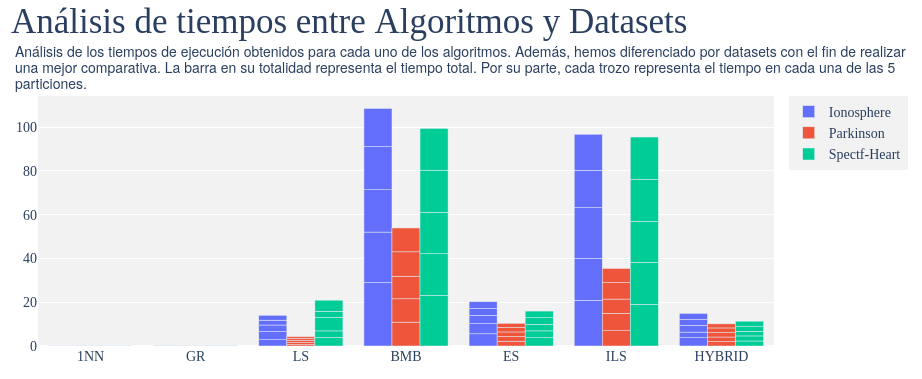
\includegraphics[scale=0.50]{Imagenes/grafica_tiempos.png}
\label{}
\end{figure} Vamos por partes. En cuanto a los \textbf{algoritmos BMB y ILS} podemos observar como presentan un runtime muchísimo mayor al de la búsqueda local. Teniendo en cuenta que estos algoritmos se basan en la aplicación reiterada de la búsqueda local, de primeras puede resultar un poco extraño. Sin embargo, esto tiene sentido debido a que en el algoritmo de la búsqueda local no se llegan a realizar todas las evaluaciones de la función objetivo. 

\begin{figure}[htp]
\centering
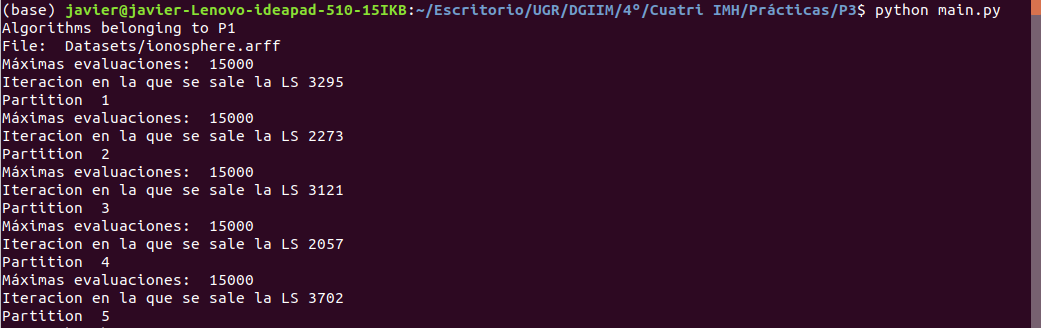
\includegraphics[scale=0.450]{Imagenes/LS_evaluaciones.png}
\caption{Nº Evaluaciones que realiza la Búsqueda Local en cada Partición en Ionosphere}
\label{}
\end{figure}

Se puede observar que la búsqueda local no llega a gastar ni un 50\% de las evaluaciones máximas totales de las que dispone. Por el contrario, hemos comprobado que para BMB, por regla general, la búsqueda local suele completar las 1000 evaluaciones correspondientes cada vez que se aplica. En el caso de ILS, hay veces en las que una ejecución de la búsqueda local no llega a esas 1000 evaluaciones. Sin embargo, suele rondar un valor muy cercano (no suele bajar de 500 evaluaciones mínimo). En caso de que se quiera comprobar esto último, basta ejecutar el archivo \textit{main.py} y comprobar las salidas por pantalla para los algoritmos de BMB y ILS. 

Pasemos a hablar de los \textbf{algoritmos ES y ILS-ES}. Podemos observar como los tiempos que obtiene el enfriamiento simulado se asemejan más a los de la búsqueda local. Para los dos primeros datasets vemos que son un poco superiores. Sin embargo, para el dataset de spectf-heart obtiene un tiempo menor. Esto tiene su causa en el tiempo que tarda la LS para la 3ª partición. Se puede apreciar que su bloque asociado consume bastante más tiempo que el resto. Por último, vemos como el híbrido mejora un poco los tiempos del ES. Con todo, cabe destacar que ninguno de estos se termina de acercar suficiente al runtime que presenta la LS para el dataset de Parkinson. 

\subsubsection{Tasa de Clasificación}

Empezamos haciendo un análisis de la comparativa entre los datasets. Para ello observamos la siguiente gráfica. Podemos ver como por regla general, el dataset de Parkinson resulta ser el más complicado de clasificar. Esto puede concluirse debido a que para todos los algoritmos sobresale por debajo la caja roja, correspondiente a los valores obtenidos para este dataset. Así mismo, podemos ver como el dataset de Ionosphere obtiene los valores menos dispersos. 

\begin{figure}[htp]
\centering
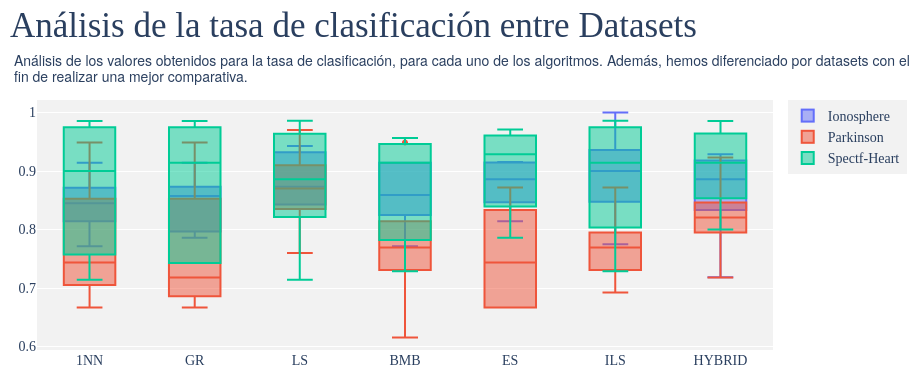
\includegraphics[scale=0.50]{Imagenes/clasificacion_graficas_datasets.png}
\label{}
\end{figure}

Pasemos ahora a estudiar la comparativa entre algoritmos. Se puede apreciar que entre los algoritmos implementados en esta práctica, son o bien el algoritmo ILS o el híbrido, ILS - ES, los que obtienen mejores valores en general. 

\begin{figure}[htp]
\centering
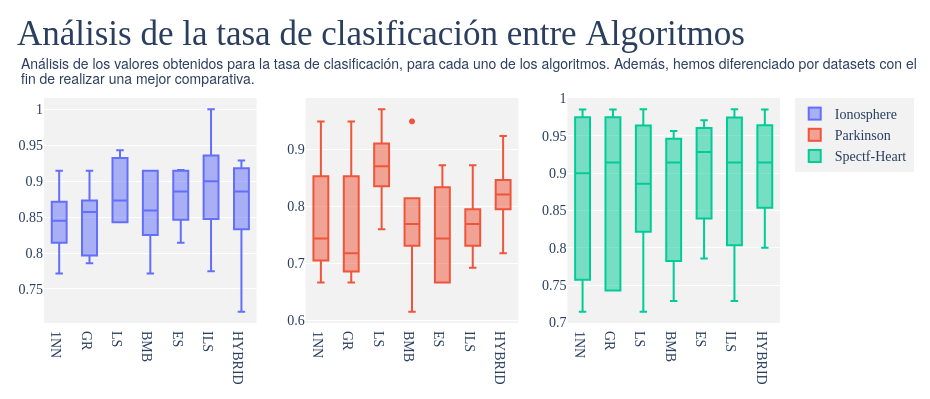
\includegraphics[scale=0.475]{Imagenes/clasificacion_graficas_algoritmos.png}
\label{}
\end{figure}

Resulta llamativa, en Ionosphere, la diferencia existente entre el valor máximo obtenido por los algoritmos LS y ILS. Aquí, el algoritmo de basado en trayectorias múltiples, debido a su capacidad de explotación de soluciones, y la de salir de óptimos locales, ha sido capaz de encontrar una solución que predice de forma perfecta sobre una de las particiones del conjunto de datos. 

\subsubsection{Tasa de Reducción}

Entre los nuevos algoritmos, vemos como sigue predominando el dataset de Parkinson como el más sencillo para reducir el vector de pesos. Es el que obtiene el valor más alto, para cada uno de los algoritmos. Recordemos que era el dataset con menor número de características. En general, suele ser spectf-heart el dataset más complicado de reducir. 

\begin{figure}[htp]
\centering
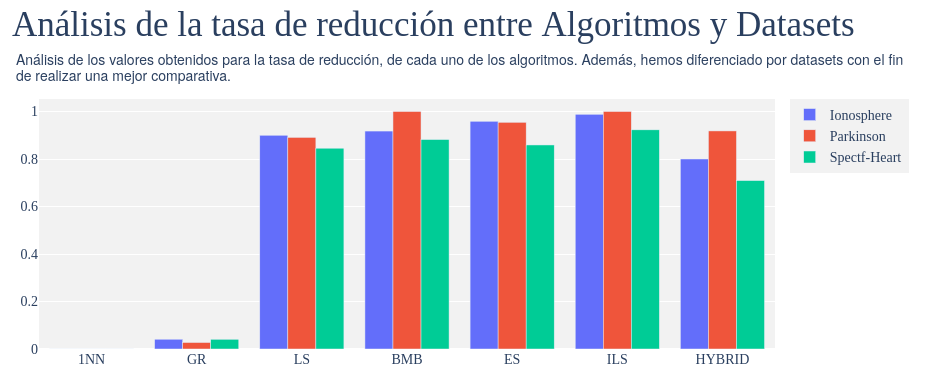
\includegraphics[scale=0.50]{Imagenes/reduccion_graficas.png}
\label{}
\end{figure}

En cuanto a la comparativa entre algoritmos, vemos que los mejores valores promedio los obtienen los algoritmos con búsqueda multiarranque BMB y ILS. Podemos ver como la mayoría de los algoritmos mejoran al valor promedio obtenido por la búsqueda local. El único que no mejora dichos valores es el híbrido, el cual obtiene además valores bastante más bajos que el resto de algoritmos implementados en esta práctica. 

\newpage
\subsubsection{Función Objetivo}

Por último, vamos a analizar los valores obtenidos para la función objetivo. En la siguiente gráfica tenemos los valores promedio para cada uno de los algoritmos. Podemos ver como los algoritmos BMB, ES y ILS han obtenido mejores valores que la búsqueda local, en todos y cada uno de los dataset. Por el contrario, el algoritmo híbrido solo ha conseguido superar a la búsqueda local en el dataset segundo, el de Parkinson. 

\begin{figure}[htp]
\centering
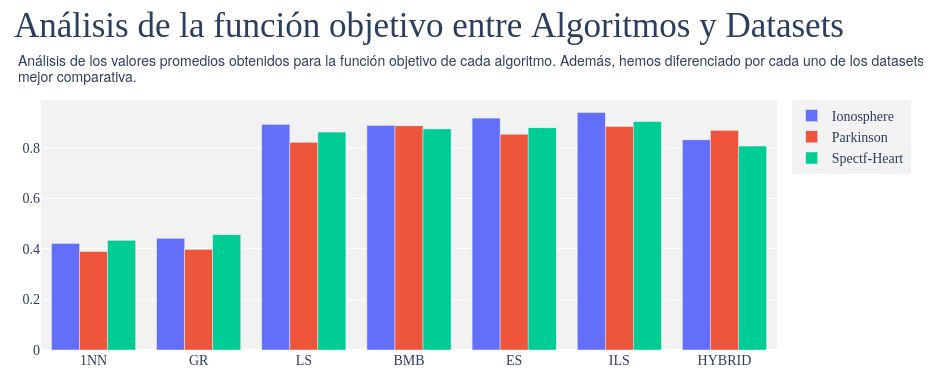
\includegraphics[scale=0.450]{Imagenes/grafica_fobjetivo.png}
\label{}
\end{figure}

\subsubsection{Análisis de convergencia}

En este último apartado vamos a estudiar como es la convergencia hacia la solución para algunos de los algoritmos implementados en esta práctica. En la siguiente gráfica tenemos la comparativa entre los algoritmos BMB y ILS.  

\begin{figure}[htp]
\centering
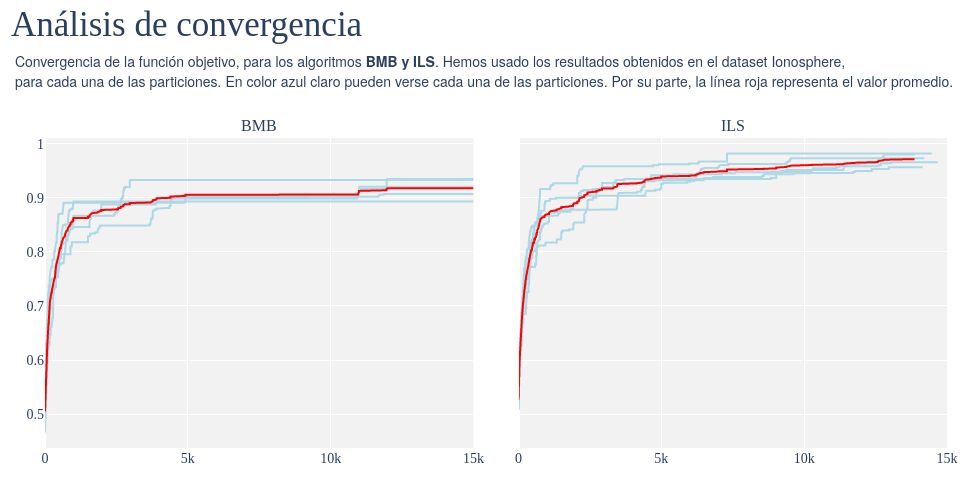
\includegraphics[scale=0.50]{Imagenes/convergencias.png}
\label{}
\end{figure}

En cuanto al algoritmo ILS, vemos como posee una convergencia más 

\end{document}